%═══════════════════════════════════════════════════════════════════════════════
\section{Controlled Simulations: Scoring the Decisions Against a Known Truth}\label{sec:simulations}
%═══════════════════════════════════════════════════════════════════════════════

The application showed the two criteria disagreeing on real data, but a
single match cannot tell which of them was right. It produced one outcome,
and an order that was cheap this time could still be the worse choice on
average. Ranking decision rules needs the distribution
that generates the outcomes, which no real match supplies. This section
therefore runs controlled simulations, in which that distribution is fixed in
advance and every rule can be scored against it.

Each simulation adds a third distribution to the model and the belief, the
truth $P_{\mathrm{true}}$. It plays no part in choosing the action. Once an
action is chosen, it is scored by its expected loss under the truth,
\[
  \mathbb E_{P_{\mathrm{true}}}\bigl[L(\delta(\mathcal E),Z)\bigr].
\]
The truth need not lie in the model, since the model is what the
decision-maker wants protection against, not a claim about where the truth
lies.

The simulations compare four ways of choosing the evidence. Two follow the
procedure of Section~\ref{sec:recipe}, one targeting the action the belief
recommends and one targeting the protective action, and by
Corollary~\ref{cor:select} each takes its target. The other two are the
likelihood ratio and the flat profile, which take whatever action the rule
selects under them. The first simulation varies how confident the belief is,
the second how much worse a losing bet is than an unnecessary hedge, and the
third how wrong the belief is. Since every distribution is known, each
expected loss is exact.

\subsection{The Likelihood Ratio Moves Against the Belief}\label{sec:sim_belief}

The first simulation asks how each rule responds as the belief grows more
confident. Keep the two-outcome loss, with the bet $L(d_1,\cdot)=(0,8)$ and
the hedge $L(d_2,\cdot)=(4,0)$, hold the truth at $(0.75,0.25)$, and let the
belief put probability $p$ on $A$.

The belief's target is the bet when betting is cheaper under the belief,
$8(1-p)\leq4p$, that is $p\geq2/3$. More confidence in $A$ makes it readier to
bet, as one would expect. The likelihood ratio against $P_0=(1/2,1/2)$ is
$\mathcal E=(2p,2(1-p))$, with certificates
\[
  C(d_1;\mathcal E)=\frac{4}{1-p},
  \qquad
  C(d_2;\mathcal E)=\frac{2}{p},
\]
so it bets only when $p\leq1/3$. The two thresholds point in opposite
directions. The likelihood ratio bets on $A$ only when the belief makes $A$
unlikely, and above $p=2/3$, where betting is genuinely cheaper, it hedges,
more firmly the more confident the belief. Figure~\ref{fig:sim_belief} shows
the actions each rule takes and their expected loss under the truth.

\begin{figure}[H]
\centering
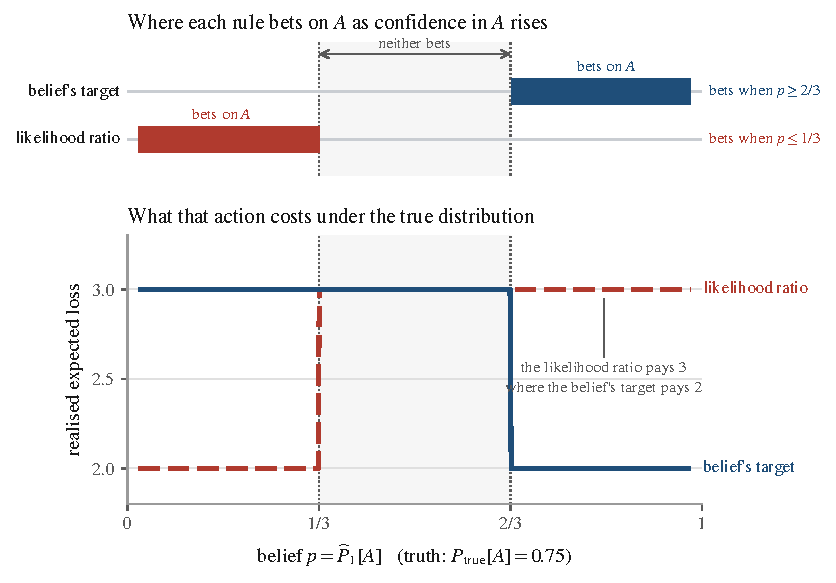
\includegraphics[width=0.92\textwidth]{sim_belief_sweep.pdf}
\caption{Actions taken and expected loss under the truth as confidence in $A$ varies. The procedure targeting the protective action and the flat profile hedge at every $p$, so only the two rules that ever bet are drawn.}\label{fig:sim_belief}
\end{figure}

This is the mechanism of Section~\ref{sec:result2} again. The likelihood
ratio puts large e-values on the outcomes the belief favours, so the rule
discounts the losses there. The bet loses only in $B$, which the belief
disfavours, so its loss is left undiscounted. That suits a profile meant as
evidence against the model, not one meant to act on a belief.

\subsection{How Wide the Disagreement Is}\label{sec:sim_window}

The second simulation varies the loss instead. Set the belief and the truth
both to $(0.75,0.25)$, so the belief is correct, and write $\ell$ for the
cost of a losing bet and $k$ for the cost of an unnecessary hedge, $8$ and $4$
in the example. With $p=0.75$, the bet is cheaper under the belief when
$\ell/k\leq p/(1-p)=3$, but the likelihood ratio selects it only when
$\ell/k\leq(1-p)/p=1/3$. In between, the likelihood ratio hedges although
betting is cheaper,
\begin{equation}
  \frac{1-p}{p}<\frac{\ell}{k}<\frac{p}{1-p},
  \qquad\text{here}\qquad \frac13<\frac{\ell}{k}<3.
  \label{eq:failure_window}
\end{equation}
The example's ratio of $2$ lies inside this window, which is why it separates
the two rules.

Since the belief is correct, the procedure targeting the belief's action has
the smallest expected loss at every ratio. What the simulation measures is the
width of the window, and \eqref{eq:failure_window} shows that it widens as the
belief grows more confident. Figure~\ref{fig:sim_window} plots the expected
losses and shades the window.

\begin{figure}[H]
\centering
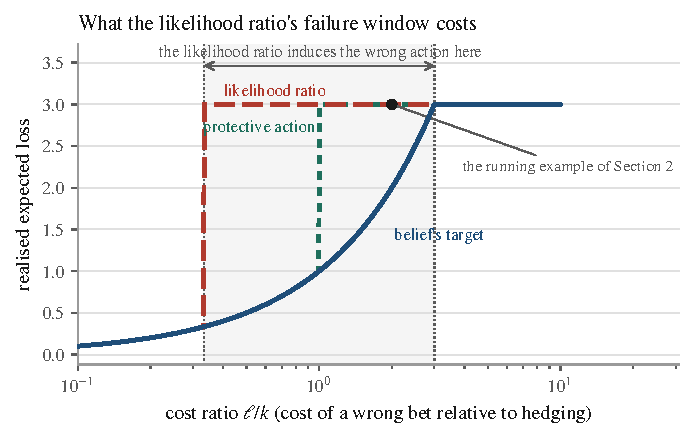
\includegraphics[width=0.92\textwidth]{sim_asymmetry_window.pdf}
\caption{Expected loss against the cost ratio $\ell/k$. Shading marks the window \eqref{eq:failure_window} in which the likelihood ratio takes the wrong action.}\label{fig:sim_window}
\end{figure}

\subsection{How Far an Optimistic Belief Can Be Trusted}\label{sec:sim_danger}

The first two simulations concern the profile: given a target, which action
does each profile lead to? This one concerns the target itself, which
Section~\ref{sec:choosing} leaves to the decision-maker's attitude toward risk.
It makes the belief wrong and asks how wrong it can be before trusting it
stops paying.

Take the three-outcome example of Section~\ref{sec:setup}, where the belief
$(0.6,0.3,0.1)$ puts only $0.1$ on the draw. Let the truth be
\[
  P_{\mathrm{true}}=\bigl(\tfrac23(1-c),\;\tfrac13(1-c),\;c\bigr),
\]
and raise the true probability $c$ of a draw from $0.01$ to $0.45$. The belief-trusting
procedure takes $d_A$ throughout, since the belief never changes, while the
guarantee-first procedure, the likelihood ratio and the flat profile all take
the insurance $d_C$. The expected losses of $d_A$ and $d_C$ under the truth
are equal at $c^*=1/4$. Below it trusting the belief costs less, and above it
insuring does.

The crossover comes well before the belief stops ranking the outcomes
correctly, since $A$ remains the most likely outcome until $c=2/5$. Ranking
correctly is not enough when the outcome the belief dismisses costs $10$. The
threshold comes from the loss table and the truth together. Draws are common
in football, so a belief that puts only $0.1$ on them may well be on the wrong
side of it.

The simulation does not say which target to name, since that depends on how
far the decision-maker trusts the belief. What it shows is what each choice
costs if the belief is wrong, which is exactly what a stated attitude toward
risk has to weigh.

Taken together, the simulations make a narrow point. The likelihood ratio can
take the wrong action even when the belief is exactly right, and over a wide
range of loss asymmetries. When the belief may be wrong, how far to trust it
depends on the loss table and the truth together, not on whether the belief
ranks the outcomes correctly.

What these simulations cannot do is show that the procedure decides better in
general, since their distributions are constructed rather than observed. That
is the price of knowing the truth at all, and Section~\ref{sec:disc_limits}
returns to it.
